\documentclass[12pt,a4paper]{article}
\usepackage[T1]{fontenc}
\usepackage[spanish,es-nodecimaldot]{babel}
\usepackage{tgtermes}
\usepackage{newtxmath}
\usepackage{amsmath}
\usepackage{textcomp}
\usepackage{graphicx}
\usepackage{geometry}
\usepackage{xcolor}
\usepackage{setspace}
\usepackage{titlesec}
\usepackage{tocloft}
\usepackage{fancyhdr}
\usepackage{enumitem}
\usepackage{hyperref}

\geometry{margin=2.5cm}

\definecolor{AzulPrincipal}{HTML}{0B2D4D}
\definecolor{AzulSecundario}{HTML}{1F5F8B}
\definecolor{OroAcento}{HTML}{C9A227}
\definecolor{GrisTexto}{HTML}{444444}

\hypersetup{
    colorlinks=true,
    linkcolor=black,
    urlcolor=black,
    citecolor=black,
    pdftitle={Plantilla de Informe},
    pdfauthor={Tu Nombre}
}

\setlength{\parindent}{1.25cm}
\setlength{\parskip}{0.25em}
\onehalfspacing

\setlist[itemize]{leftmargin=2.8em, labelsep=0.8em, topsep=0.35em, itemsep=0.2em}
\setlist[enumerate]{leftmargin=1.7em, topsep=0.35em, itemsep=0.2em}

\titleformat{\section}[hang]{\fontsize{18pt}{22pt}\selectfont\normalfont\color{black}}{\thesection.}{0.8em}{}
\titleformat{\subsection}[hang]{\fontsize{14pt}{17pt}\selectfont\normalfont\color{black}}{\thesubsection}{0.8em}{}

\renewcommand{\cftsecfont}{\normalfont}
\renewcommand{\cftsecpagefont}{\normalfont}
\renewcommand{\cftsubsecfont}{\normalfont}
\renewcommand{\cftsubsecpagefont}{\normalfont}
\renewcommand{\cftsecleader}{\cftdotfill{\cftdotsep}}
\renewcommand{\cftsubsecleader}{\cftdotfill{\cftdotsep}}
\renewcommand{\contentsname}{Índice}
\renewcommand{\cfttoctitlefont}{\hfill\normalfont\fontsize{18pt}{22pt}\selectfont}
\renewcommand{\cftaftertoctitle}{\hfill}

\titlespacing*{\section}{0pt}{1.1em}{0.55em}
\titlespacing*{\subsection}{0pt}{0.9em}{0.35em}

\setlength{\headheight}{30pt}

\pagestyle{fancy}
\fancyhf{}
\lhead{\small\textcolor{black!65}{\Laboratorio: \Tema}}
\rhead{}
\cfoot{\small\textcolor{black}{\thepage}}
\renewcommand{\headrulewidth}{0.4pt}
\renewcommand{\headrule}{\hbox to\headwidth{\color{black!65}\leaders\hrule height \headrulewidth\hfill}}
\renewcommand{\footrulewidth}{0pt}

\providecommand{\Universidad}{UNIVERSIDAD NACIONAL DE INGENIERÍA}
\providecommand{\Facultad}{FACULTAD DE CIENCIAS}
\providecommand{\Escuela}{ESCUELA DE FÍSICA}
\providecommand{\Curso}{CIRCUITOS ELÉCTRICOS ANALÓGICOS}
\providecommand{\Seccion}{SECCIÓN A}
\providecommand{\NumeroLaboratorio}{X}
\providecommand{\Laboratorio}{LABORATORIO N\textdegree{} \NumeroLaboratorio}
\providecommand{\Tema}{TÍTULO DE LA PRÁCTICA}
\providecommand{\RutaLogo}{logo.PNG}
\providecommand{\IntegrantesBloque}{%
\begin{enumerate}[leftmargin=1.8em,label=\arabic*.]
    \item Integrante 1 -- código
    \item Integrante 2 -- código
\end{enumerate}}
\providecommand{\FechaRealizacion}{Fecha de realización: dd de mes de aaaa - hh:mm}
\providecommand{\Ciudad}{LIMA - PERU}

\newcommand{\ConfigurarInforme}[3]{%
    \renewcommand{\NumeroLaboratorio}{#1}%
    \renewcommand{\Tema}{#2}%
    \renewcommand{\FechaRealizacion}{#3}%
}

\newcommand{\ConfigurarIntegrantes}[1]{%
    \renewcommand{\IntegrantesBloque}{#1}%
}

\providecommand{\tituloSeccion}[1]{\section{#1}}

\providecommand{\makeInformePortada}{%
\begin{titlepage}
    \thispagestyle{empty}
    \vspace*{0.65cm}
    \begin{center}
        {\Large\bfseries\color{OroAcento} \Universidad}\par
        \vspace{0.45cm}
        {\Large\bfseries\color{AzulPrincipal} \Facultad}\par
        \vspace{0.25cm}
        {\Large\bfseries\color{AzulPrincipal} \Escuela}\par
    \end{center}

    \vspace{0.1cm}
    \begin{center}
        \includegraphics[width=0.4\textwidth]{\RutaLogo}%
    \end{center}

    \vspace{0.01cm}
    \begin{center}
        {\Large\bfseries\color{AzulPrincipal} \Curso}\par
        \vspace{0.35cm}
        {\Large\bfseries\color{red} \Seccion}\par
    \end{center}

    \vspace{0.1cm}
    \begin{center}
        {\large\bfseries \Laboratorio: \Tema}\par
    \end{center}

    \vspace{0.55cm}
    \noindent{\large\textbf{INTEGRANTES DE LA MESA:} 2}\par
    \vspace{0.35cm}
    \begingroup
    \leftskip=1.15cm
    \rightskip=1.15cm
    \parindent=0pt
    \IntegrantesBloque
    \endgroup

    \vspace{0.55cm}
    \begin{center}
        {\FechaRealizacion}\par
    \end{center}

    \vfill

    \begin{center}
        {\large\bfseries \Ciudad}
    \end{center}
\end{titlepage}
}
\usepackage{tikz}
\usepackage{pgfplots}
\pgfplotsset{compat=1.18}
\renewcommand{\RutaLogo}{../../PLANTILLA/logo.PNG}
\graphicspath{{Imagenes/}}
\ConfigurarInforme{5}{FILTROS RC}{Fecha de realización del Laboratorio N\textdegree{}5: 21 de Abril del 2026}

% Inicio del informe
\begin{document}
\makeInformePortada
\setcounter{page}{1}
\tableofcontents
\newpage

% Contenido del informe
\tituloSeccion{Objetivos}
\subsection{Objetivo general}
\begin{itemize}
	\item Estudiar y analizar el comportamiento de un circuito RC como filtro en frecuencia.
\end{itemize}

\subsection{Objetivos específicos}
\begin{itemize}
	\item Medir y analizar la relación entre el voltaje de entrada y salida a diferentes frecuencias  en filtros de señales según la frecuencia de tipos pasa-baja y pasa-alta.
	\item Calcular la frecuencia de corte y la constante de tiempo de los filtros RC.
	\item Observar las condiciones bajo las cuales el filtro RC actúa como integrador o derivador de señales.
\end{itemize}

\tituloSeccion{Fundamento teórico}

\subsection{Filtro pasa-baja RC}
Un filtro pasa-baja RC se muestra en la figura \ref{fig:pasa-baja} y permite el paso de señales de baja frecuencia y atenúa progresivamente las señales de mayor frecuencia. En este circuito, la salida se toma en el capacitor. 
\begin{figure}[H]
	\centering
	
\includegraphics[width=0.4\linewidth]{Imagen1.png}
	\caption{Filtro pasa-baja RC.}
	\label{fig:pasa-baja}
\end{figure}
Su frecuencia de corte está dada por
\begin{equation}
	f_c = \frac{1}{2\pi RC}
    \label{eq:frecuencia-corte}
\end{equation}
y la magnitud de la función de transferencia puede expresarse como
\begin{equation}
	T = \left|\frac{V_{out}}{V_{in}}\right| = \frac{1}{\sqrt{1 + \left(\frac{f}{f_c}\right)^2}}
\end{equation}
La fase asociada a la salida es
\begin{equation}
	\alpha = -\arctan\left(\frac{f}{f_c}\right)
\end{equation}
Cuando $f = f_c$, se cumple $T = 1/\sqrt{2} \approx 0,707$ y $\alpha = -45^\circ$.

\subsection{Filtro pasa-alta RC}
Un filtro pasa-alta RC se muestra en la figura \ref{fig:pasa-alta} y permite el paso de señales de alta frecuencia y atenúa las de baja frecuencia. En este caso, la salida se toma en el resistor.
\begin{figure}[H]
    \centering
    
\includegraphics[width=0.4\linewidth]{Imagen2.png}
    \caption{Filtro pasa-alta RC.}
    \label{fig:pasa-alta}
\end{figure}
 La frecuencia de corte es la misma expresión:
\begin{equation}
	f_c = \frac{1}{2\pi RC}
\end{equation}
La magnitud de la función de transferencia es
\begin{equation}
	T = \left|\frac{V_{out}}{V_{in}}\right| = \frac{1}{\sqrt{1 + \left(\frac{f_c}{f}\right)^2}}
\end{equation}
y la fase queda dada por
\begin{equation}
	\alpha = \arctan\left(\frac{f_c}{f}\right)
\end{equation}
Para $f = f_c$ también se obtiene $T = 0,707$ y $\alpha = 45^\circ$.

\subsection{Filtro pasabanda}
Un filtro pasabanda permite el paso de una banda de frecuencias intermedia y atenúa las frecuencias por debajo y por encima de ese rango. Una forma simple de implementarlo consiste en combinar un filtro pasa-alta con un filtro pasa-baja. Si $f_{c_a}$ es la frecuencia de corte inferior y $f_{c_b}$ la frecuencia de corte superior, debe cumplirse
\begin{equation}
	f_{c_a} < f_{c_b}
\end{equation}
La respuesta global presenta una región de mayor amplitud entre ambas frecuencias de corte.

\newpage
\tituloSeccion{Materiales e indicaciones}
\begin{itemize}
	\item Multímetro: Instrumento de medición utilizado para verificar los valores de resistencia de los componentes, así como para medir voltajes en el circuito. 
	\item Osciloscopio: Instrumento de medición que permite visualizar en tiempo real la forma de onda de las señales de entrada y salida del circuito. Se empleó para medir voltajes pico, comparar amplitudes y determinar el desfase entre canales mediante la diferencia temporal entre señales, especialmente en la frecuencia de corte.
	\item Generador de señales: Equipo utilizado para excitar el circuito RC con señales periódicas de amplitud controlada (principalmente sinusoidal) y frecuencia ajustable.
    \item Resistencias: Son componentes que limitan el flujo de corriente en un circuito. Para su uso, se deben identificar sus valores utilizando el código de colores o un multímetro, y conectarlas en el circuito según sea necesario.
    \item Capacitores: Son componentes que almacenan energía eléctrica en forma de campo eléctrico. Para su uso, se deben identificar sus valores utilizando el código de colores o un multímetro, y conectarlos en el circuito según sea necesario.
    \item Protoboard: Es una placa de pruebas que permite realizar conexiones temporales sin necesidad de soldar. Para su uso, se deben insertar los componentes en las filas y columnas correspondientes, y realizar las conexiones utilizando cables de puente.
\end{itemize}

\tituloSeccion{Procedimiento experimental}

\subsection{Paso 1: Filtro pasa-baja RC}
\begin{enumerate}
	\item Se conectaron los instrumentos de medición: el osciloscopio para visualizar las señales de entrada y salida, el generador de señales para proporcionar la señal de prueba, y el multímetro para verificar los valores de los componentes. Se armó el circuito pasa-baja RC según la figura \ref{fig:circuito-pasa-baja} cambiando los valores de la resistencia y el capacitor a $(10,0 \pm 0,1)\,\mathrm{k}\Omega$ y $(3,98 \pm 0,01)\,\mathrm{nF}$, respectivamente.
    \begin{figure}[H]
        \centering
        
\includegraphics[width=0.4\linewidth]{Imagen3.png}
        \caption{Circuito pasa-baja RC.}
        \label{fig:circuito-pasa-baja}
    \end{figure}
    \item Luego se calculó la constante de tiempo $\tau = RC$ y la frecuencia de corte teórica usando usando la ecuación \ref{eq:frecuencia-corte}. Los datos fueron registrados en la Tabla \ref{tab:tabla-5-1}.
	\item Se aplicó una señal sinusoidal de amplitud pico a pico de 5 V y se midió el voltaje de salida para frecuencias cercanas a la frecuencia de corte, con los valores obtenidos se calculó la razón $V_{out}/V_{in}$ y se registraron los datos en la Tabla \ref{tab:pasa-baja}.
	\item Se ajustó la frecuencia de entrada al valor de corte del filtro pasa-baja.
	\item Con ayuda de las funciones del osciloscopio, se obtuvo la elipse de Lissajous y midiendo las divisiones entre el punto más alto y el corte de la gráfica con el eje Y se determinó el desfase según la fórmula
    \begin{equation}
        \alpha = \arcsen\left(\frac{Y_0}{Y_{\max}}\right) = \arcsen\left(\frac{\text{Intersección con el eje Y}}{\text{Amplitud máxima en Y}}\right)
    \end{equation}
	\item Se comparó el resultado experimental con el módulo del valor teórico del angulo de desfase en la frecuencia de corte, que es $45^\circ$. Los resultados se registraron en la Tabla \ref{tab:tabla-5-3}.
\end{enumerate}

\subsection{Paso 2: Filtro pasa-alta RC}
\begin{enumerate}
	\item Se armó el circuito pasa-alta RC según la Figura \ref{fig:circuito-pasa-alta} con un capacitor de $(3,98 \pm 0,01)\,\mathrm{nF}$ y una resistencia de $(15,59 \pm 0,01)\,\mathrm{k}\Omega$.
	\begin{figure}[H]
        \centering
        
\includegraphics[width=0.4\linewidth]{Imagen4.png}
        \caption{Circuito pasa-alta RC.}
        \label{fig:circuito-pasa-alta}
    \end{figure}
    \item Se realizó el mismo procedimiento que en el filtro pasa-baja y los datos fueron anotados en las tablas \ref{tab:tabla-5-4} y \ref{tab:pasa-alta}.
\end{enumerate}

\newpage
\tituloSeccion{Análisis de datos}

\subsection{Filtro pasa-baja RC}

\textbf{Datos reales:}
\begin{itemize}
	\item $R = (10,0 \pm 0,1)\,\mathrm{k}\Omega$
	\item $C = (3,98 \pm 0,01)\,\mathrm{nF}$
\end{itemize}

\begin{table}[H]
	\centering
	\fontsize{10pt}{12pt}\selectfont
	\renewcommand{\arraystretch}{1.2}
	\setlength{\tabcolsep}{6pt}
	{\begin{tabular}{|C{3.2cm}|C{4cm}|}
	\hline
	\textbf{$\tau$ (s) Calculado} & \textbf{$f_c$ (Hz) Calculado}\\
	\hline
	$39,8\,\mu$s & $3988,87$\\
	\hline
	\end{tabular}}
	\caption{Constante de tiempo y frecuencia de corte del filtro pasa-baja.}
	\label{tab:tabla-5-1}
\end{table}

\begin{table}[H]
	\centering
	\fontsize{10pt}{12pt}\selectfont
	\renewcommand{\arraystretch}{1.2}
	\setlength{\tabcolsep}{6pt}
	{\begin{tabular}{|C{3cm}|C{3cm}|C{3cm}|}
	\hline
		\textbf{$V_{out}$ (V) ($\pm 0{,}01\ \mathrm{V}$)} & \textbf{$f$ (Hz)} & \textbf{$V_{out}/V_{in}$} \\
	\hline
	$4,51$ & $2000$ & $0,902$ \\
	\hline
	$4,28$ & $2500$ & $0,856$ \\
	\hline
	$4,00$ & $3000$ & $0,800$ \\
	\hline
	$3,76$ & $3500$ & $0,752$ \\
	\hline
	$3,56$ & $4000$ & $0,712$ \\
	\hline
	$3,37$ & $4500$ & $0,674$ \\
	\hline
	$3,13$ & $5000$ & $0,626$ \\
	\hline
	$2,93$ & $5500$ & $0,586$ \\
	\hline
	$2,77$ & $6000$ & $0,554$ \\
	\hline
	$2,69$ & $6500$ & $0,538$ \\
	\hline
	\end{tabular}}
	\caption{Medición de voltaje de salida y relación de amplitudes en el filtro pasa-baja.}
	\label{tab:pasa-baja}
\end{table}

\begin{figure}[H]
	\centering
	\begin{tikzpicture}
		\begin{semilogxaxis}[
			width=0.82\linewidth,
			height=0.45\linewidth,
			title={Filtro pasa-baja RC},
			xlabel={$f$ (Hz)},
			ylabel={$V_{out}/V_{in}$},
			title style={font=\small},
			xlabel style={font=\small},
			ylabel style={font=\small},
			tick label style={font=\scriptsize},
			xmin=1800, xmax=7000,
			ymin=0.5, ymax=0.95,
			grid=both,
			minor grid style={gray!25},
			major grid style={gray!50},
			tick align=outside,
			legend pos=south west,
			legend style={font=\scriptsize, draw=none, fill=none},
			every axis plot/.append style={line width=1pt}
		]
			\addplot+[mark=*, mark size=2pt, error bars/.cd, y dir=both, y explicit] coordinates {
				(2000,0.902) +- (0,0.01)
				(2500,0.856) +- (0,0.01)
				(3000,0.800) +- (0,0.01)
				(3500,0.752) +- (0,0.01)
				(4000,0.712) +- (0,0.01)
				(4500,0.674) +- (0,0.01)
				(5000,0.626) +- (0,0.01)
				(5500,0.586) +- (0,0.01)
				(6000,0.554) +- (0,0.01)
				(6500,0.538) +- (0,0.01)
			};
			\addlegendentry{Experimental (barras amplificadas 5\texttimes{} para visualización)}
			\addplot+[dashed, mark=none, black!70, domain=1800:7000, samples=200] {1/sqrt(1 + (x/3988.87)^2)};
			\addlegendentry{Teórica}
		\end{semilogxaxis}
	\end{tikzpicture}
	\caption{Gráfica semilogarítmica de $V_{out}/V_{in}$ vs. $f$ para el filtro pasa-baja.}
	\label{fig:semilog-pasa-baja}
\end{figure}

\textbf{ANÁLISIS:} Los datos muestran una disminución progresiva de $V_{out}/V_{in}$ conforme la frecuencia aumenta. El valor experimental se aproxima a $0,707$ alrededor de $4000\,\mathrm{Hz}$, por lo que la frecuencia de corte observada concuerda con la calculada teóricamente. Esto confirma el comportamiento típico del filtro pasa-baja.

\bigskip
\begin{table}[H]
	\centering
	\fontsize{10pt}{12pt}\selectfont
	\renewcommand{\arraystretch}{1.2}
	\setlength{\tabcolsep}{6pt}
	{\begin{tabular}{|C{3cm}|C{3cm}|C{3cm}|}
	\hline
	\textbf{$\alpha$ (°) Calculado} & \textbf{$\alpha$ (°) Medido} & \textbf{$\%$ error relativo} \\
	\hline
	$45$ & $46,24$ & $2,75\%$ \\
	\hline
	\end{tabular}}
	\caption{Desfase en la frecuencia de corte del filtro pasa-baja.}
	\label{tab:tabla-5-3}
\end{table}

\textbf{ANÁLISIS:} El desfase medido en la frecuencia de corte es muy cercano al valor teórico de $45^\circ$, con un error relativo de $2,75\%$. La diferencia puede atribuirse a la forma de medida, que fue, en esencia, una aproximación visual a través de la elipse de Lissajous, lo que introduce cierta incertidumbre en la determinación del ángulo.

\subsection{Filtro pasa-alta RC}

\textbf{Datos reales:}
\begin{itemize}
	\item $R = (15,59 \pm 0,01)\,\mathrm{k}\Omega$
	\item $C = (3,98 \pm 0,01)\,\mathrm{nF}$
\end{itemize}

\begin{table}[H]
	\centering
	\fontsize{10pt}{12pt}\selectfont
	\renewcommand{\arraystretch}{1.2}
	\setlength{\tabcolsep}{6pt}
	{\begin{tabular}{|C{3.2cm}|C{4cm}|}
	\hline
	\textbf{$\tau$ (s) Calculado} & \textbf{$f_c$ (Hz) Calculado}\\
	\hline
	$77,89\,\mu$s & $2043,37$\\
	\hline
	\end{tabular}}
	\caption{Constante de tiempo y frecuencia de corte del filtro pasa-alta.}
	\label{tab:tabla-5-4}
\end{table}

\begin{table}[H]
	\centering
	\fontsize{10pt}{12pt}\selectfont
	\renewcommand{\arraystretch}{1.2}
	\setlength{\tabcolsep}{6pt}
	{\begin{tabular}{|C{3cm}|C{3cm}|C{3cm}|}
	\hline
		\textbf{$V_{out}$ (V) ($\pm 0{,}01\ \mathrm{V}$)} & \textbf{$f$ (Hz)} & \textbf{$V_{out}/V_{in}$} \\
	\hline
	$1,21$ & $500$ & $0,242$ \\
	\hline
	$2,18$ & $1000$ & $0,436$ \\
	\hline
	$2,93$ & $1500$ & $0,586$ \\
	\hline
	$3,46$ & $2000$ & $0,692$ \\
	\hline
	$3,82$ & $2500$ & $0,764$ \\
	\hline
	$4,06$ & $3000$ & $0,812$ \\
	\hline
	$4,26$ & $3500$ & $0,852$ \\
	\hline
	$4,40$ & $4000$ & $0,880$ \\
	\hline
	$4,49$ & $4500$ & $0,898$ \\
	\hline
	$4,63$ & $5000$ & $0,926$ \\
	\hline
	\end{tabular}}
	\caption{Medición de voltaje de salida y relación de amplitudes en el filtro pasa-alta.}
	\label{tab:pasa-alta}
\end{table}

\begin{figure}[H]
	\centering
	\begin{tikzpicture}
		\begin{semilogxaxis}[
			width=0.82\linewidth,
			height=0.45\linewidth,
			title={Filtro pasa-alta RC},
			xlabel={$f$ (Hz)},
			ylabel={$V_{out}/V_{in}$},
			title style={font=\small},
			xlabel style={font=\small},
			ylabel style={font=\small},
			tick label style={font=\scriptsize},
			xmin=450, xmax=5500,
			ymin=0.2, ymax=0.95,
			grid=both,
			minor grid style={gray!25},
			major grid style={gray!50},
			tick align=outside,
			legend pos=south east,
			legend style={font=\scriptsize, draw=none, fill=none},
			every axis plot/.append style={line width=1pt}
		]
			\addplot+[mark=*, mark size=2pt, error bars/.cd, y dir=both, y explicit] coordinates {
				(500,0.242) +- (0,0.01)
				(1000,0.436) +- (0,0.01)
				(1500,0.586) +- (0,0.01)
				(2000,0.692) +- (0,0.01)
				(2500,0.764) +- (0,0.01)
				(3000,0.812) +- (0,0.01)
				(3500,0.852) +- (0,0.01)
				(4000,0.880) +- (0,0.01)
				(4500,0.898) +- (0,0.01)
				(5000,0.926) +- (0,0.01)
			};
			\addlegendentry{Experimental (barras amplificadas 5\texttimes{})}
			\addplot+[dashed, mark=none, black!70, domain=450:5500, samples=200] {1/sqrt(1 + (2043.37/x)^2)};
			\addlegendentry{Teórica}
		\end{semilogxaxis}
	\end{tikzpicture}
	\caption{Gráfica semilogarítmica de $V_{out}/V_{in}$ vs. $f$ para el filtro pasa-alta.}
	\label{fig:semilog-pasa-alta}
\end{figure}

\textbf{ANÁLISIS:} La relación $V_{out}/V_{in}$ aumenta conforme crece la frecuencia, lo que coincide con el comportamiento esperado de un filtro pasa-alta. Cerca de $2000\,\mathrm{Hz}$ la razón experimental se aproxima a $0,707$, por lo que la frecuencia de corte observada coincide con la predicción teórica.

\bigskip
\begin{table}[H]
	\centering
	\fontsize{10pt}{12pt}\selectfont
	\renewcommand{\arraystretch}{1.2}
	\setlength{\tabcolsep}{6pt}
	{\begin{tabular}{|C{3cm}|C{3cm}|C{3cm}|}
	\hline
	\textbf{$\alpha$ (°) Calculado} & \textbf{$\alpha$ (°) Medido} & \textbf{$\%$ error relativo} \\
	\hline
	$45$ & $45,58$ & $1,28\%$ \\
	\hline
	\end{tabular}}
	\caption{Desfase en la frecuencia de corte del filtro pasa-alta.}
	\label{tab:tabla-5-6}
\end{table}

\textbf{ANÁLISIS:} El desfase medido en la frecuencia de corte del filtro pasa-alta presenta la misma tendencia que el filtro pasa-baja, con un valor cercano a los $45^\circ$ teóricos y un error relativo de $1,28\%$. Nuevamente, la aproximación visual a través de la elipse de Lissajous es la principal fuente de incertidumbre en esta medición.


\tituloSeccion{Actividades adicionales}

\subsection{¿Por qué el filtro pasa-baja funciona como integrador a frecuencias mucho mayores que la frecuencia de corte?}
En un filtro pasa-baja RC la salida se toma en el capacitor. Cuando la frecuencia de entrada es mucho mayor que la frecuencia de corte ($f \gg f_c$), la señal varía muy rápidamente en comparación con el tiempo característico $RC$. En este régimen, el capacitor no puede seguir dichas variaciones rápidas, por lo que la tensión en él permanece pequeña y cambia de forma más suave que la señal de entrada. Como consecuencia, el circuito atenúa fuertemente las componentes de alta frecuencia.

Matemáticamente, en esta condición la función de transferencia se aproxima a:
\begin{equation}
H(j\omega) \approx \frac{1}{j\omega RC}
\end{equation}

lo cual corresponde al comportamiento de un integrador en el dominio de la frecuencia.

Equivalentemente, a partir de la ecuación diferencial del circuito:
\begin{equation}
RC \frac{dV_{out}}{dt} + V_{out} = V_{in}
\end{equation}

y considerando que $V_{out}$ es pequeño frente a $V_{in}$ a altas frecuencias, se obtiene la aproximación:
\begin{equation}
RC \frac{dV_{out}}{dt} \approx V_{in}
\end{equation}

lo que implica que la salida varía según la pendiente impuesta por la entrada, es decir, el circuito se comporta como un integrador.
\subsection{¿Por qué el filtro pasa-alta funciona como derivador a frecuencias mucho menores que la frecuencia de corte?}

En el filtro pasa-alta RC la salida se mide en la resistencia. Cuando la frecuencia de trabajo es mucho menor que la frecuencia de corte ($f \ll f_c$), la señal varía muy lentamente en comparación con el tiempo característico $RC$. En este régimen, el capacitor tiene una reactancia elevada, lo que limita fuertemente la corriente en el circuito. Como consecuencia, la caída de tensión en la resistencia (salida) es pequeña.

Sin embargo, la corriente en el circuito depende de qué tan rápido cambia la señal de entrada. Por ello, la tensión en la resistencia resulta proporcional a la rapidez de variación de la señal de entrada.

Matemáticamente, en esta condición la función de transferencia se aproxima a:
\begin{equation}
H(j\omega) \approx j\omega RC
\end{equation}

lo cual corresponde al comportamiento de un derivador en el dominio de la frecuencia.

Equivalentemente, a partir de la ecuación del circuito:
\begin{equation}
V_{out} = R i = RC \frac{dV_{in}}{dt}
\end{equation}

se observa que la salida es proporcional a la derivada temporal de la entrada. Esto implica que el circuito resalta cambios rápidos en la señal: transiciones abruptas generan una mayor respuesta, mientras que variaciones lentas producen una salida pequeña.

\subsection{Filtro pasabanda formado por un pasa-alta y un pasa-baja}

Un filtro pasabanda puede obtenerse conectando en cascada un filtro pasa-alta y un filtro pasa-baja. Cada etapa atenúa una región distinta del espectro:

\begin{itemize}
    \item El pasa-alta atenúa las frecuencias por debajo de su frecuencia de corte inferior $f_{c_a}$.
    \item El pasa-baja atenúa las frecuencias por encima de su frecuencia de corte superior $f_{c_b}$.
\end{itemize}

Para que exista una banda de paso bien definida, debe cumplirse:
\begin{equation}
f_{c_a} < f_{c_b}
\end{equation}

En el intervalo intermedio ($f_{c_a} < f < f_{c_b}$), ambas etapas permiten el paso de la señal, por lo que la salida conserva una amplitud significativa.

La respuesta global del sistema se obtiene como el producto de ambas funciones de transferencia:
\begin{equation}
H_{bp}(j\omega) = H_{pa}(j\omega)\,H_{pb}(j\omega)
\end{equation}

Por ello, la curva de magnitud presenta tres regiones características: fuerte atenuación a bajas frecuencias, una banda de paso en frecuencias intermedias, y nuevamente atenuación a altas frecuencias.
\tituloSeccion{Conclusiones}
\begin{itemize}
	\item Se verificó experimentalmente el comportamiento esperado de los filtros RC pasa-baja y pasa-alta, observando la variación de la amplitud con la frecuencia.
	\item Las frecuencias de corte obtenidas a partir de los componentes reales concuerdan con los valores observados en las mediciones de amplitud y desfase.
	\item Los desfases medidos en la frecuencia de corte fueron muy cercanos a los valores teóricos de $45^\circ$, con errores relativos pequeños.
\end{itemize}

\tituloSeccion{Bibliografía}
\begin{enumerate}[label={[\arabic*]}]
	\item R. L. Boylestad, \textit{Introducción al análisis de circuitos}, 12.\textsuperscript{a} ed. México: Pearson Education/Prentice Hall, 2010.
    \item UNI-FC, \textit{Circuitos Electrónicos Analógicos: Guía de laboratorio del experimento 5}. Lima, Perú, 2026.
\end{enumerate}

\tituloSeccion{Anexos}
\begin{figure}[H]
    \centering
    \begin{minipage}{0.48\linewidth}
        \centering
        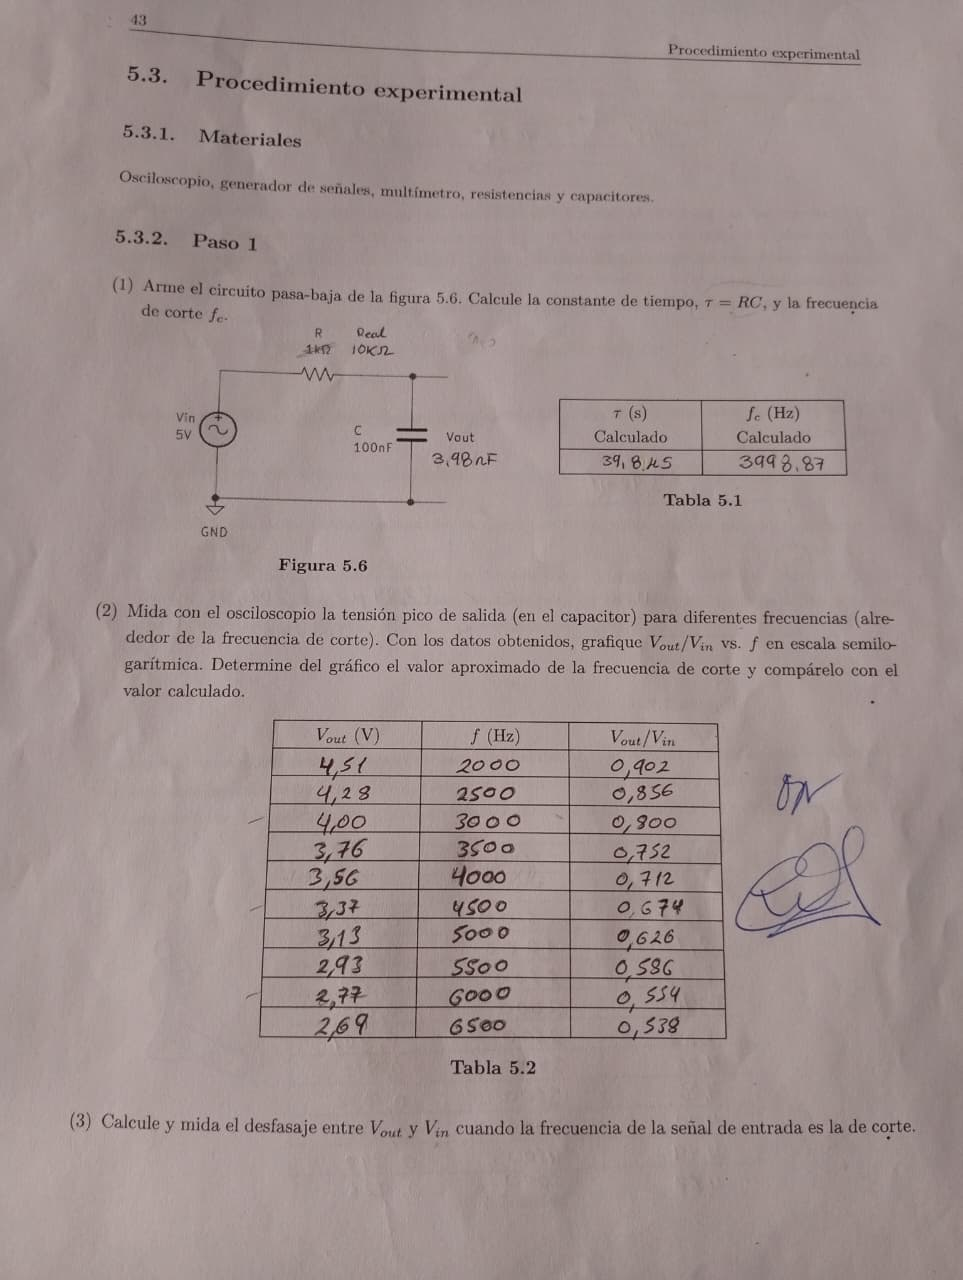
\includegraphics[width=\linewidth]{Imagen5.jpeg}
        \caption{Anexo 1: PASO.}
        \label{anexo1}
    \end{minipage}
    \hspace{0.02\linewidth}
    \begin{minipage}{0.48\linewidth}
        \centering
        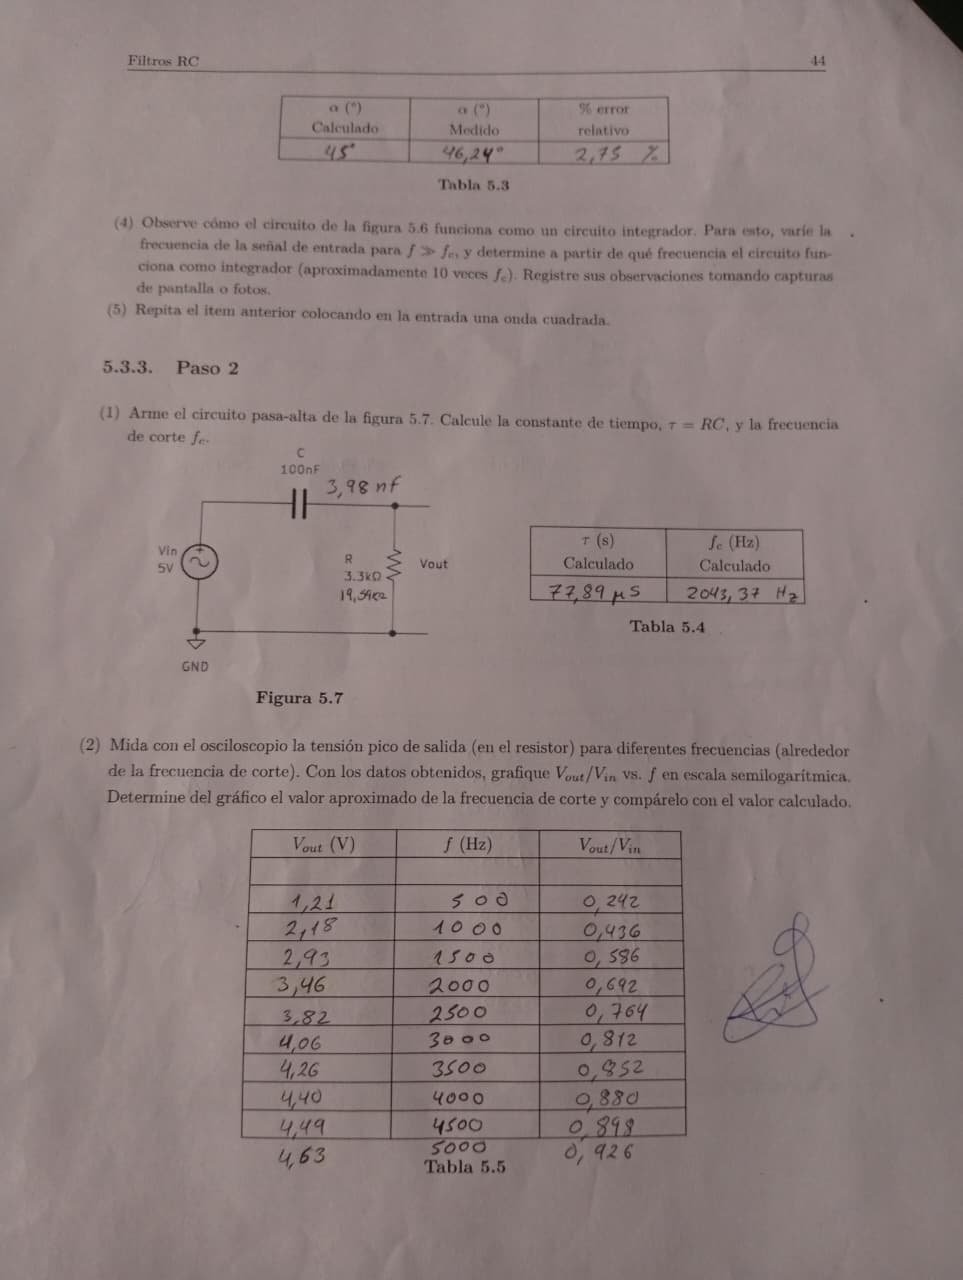
\includegraphics[width=\linewidth]{Imagen6.jpeg}
        \caption{Anexo 2: PASO 2.}
        \label{anexo2}
    \end{minipage}
\end{figure}

\begin{figure}[H]
    \centering
    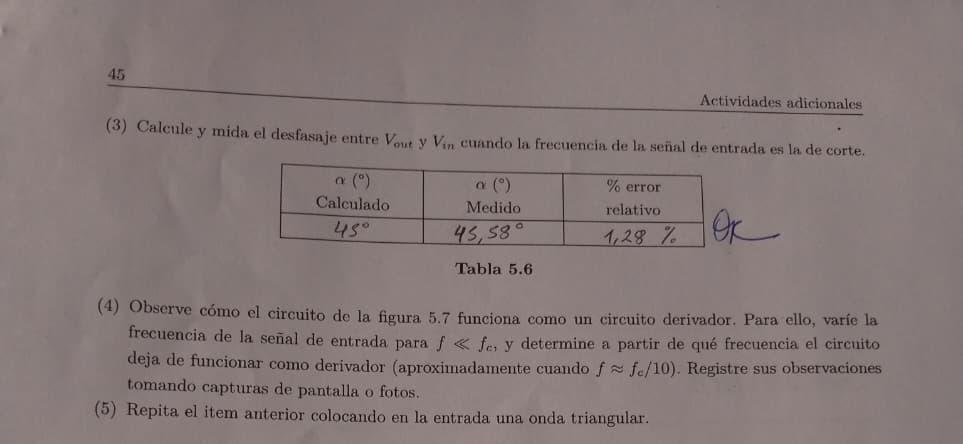
\includegraphics[width=0.6\linewidth]{Imagen7.jpeg}
    \caption{Anexo 3: PASO 2.}
    \label{anexo3}
\end{figure}

\end{document}